\chapter{Reporting}
Reporting is a core concept of Varroa.
Its purpose is determine the result values of a Varroa test and output them in a verifiable document.
For that reason there are entities that observe the parts of Varroa that execute the scenario.
These exist on different hierarchy levels.
Figure \ref{fig:ReportingArchitecture} shows the entities that are responsible for observing the actions that have taken place as well as their hierarchy.

\section{Reporting Architecture}
\begin{figure}[H]
	\begin{center}
		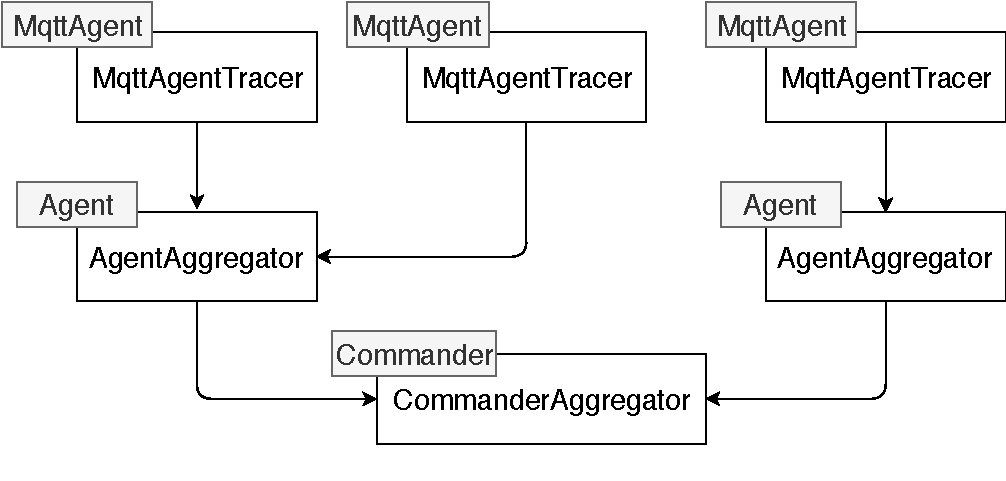
\includegraphics[scale=0.8]{Resources/PDF/ReportingArchitecture}
		\caption{Reporting Architecture}
		\label{fig:ReportingArchitecture}
	\end{center}
\end{figure}


%\subsection{Actions}

\subsection{Aggregation of Actions}

\section{Metrics}

\subsection{Time needed}

%TODO more different types of Metrics


